\section{Mental Death}

\begin{wrapfigure}{rt}{.35\textwidth}
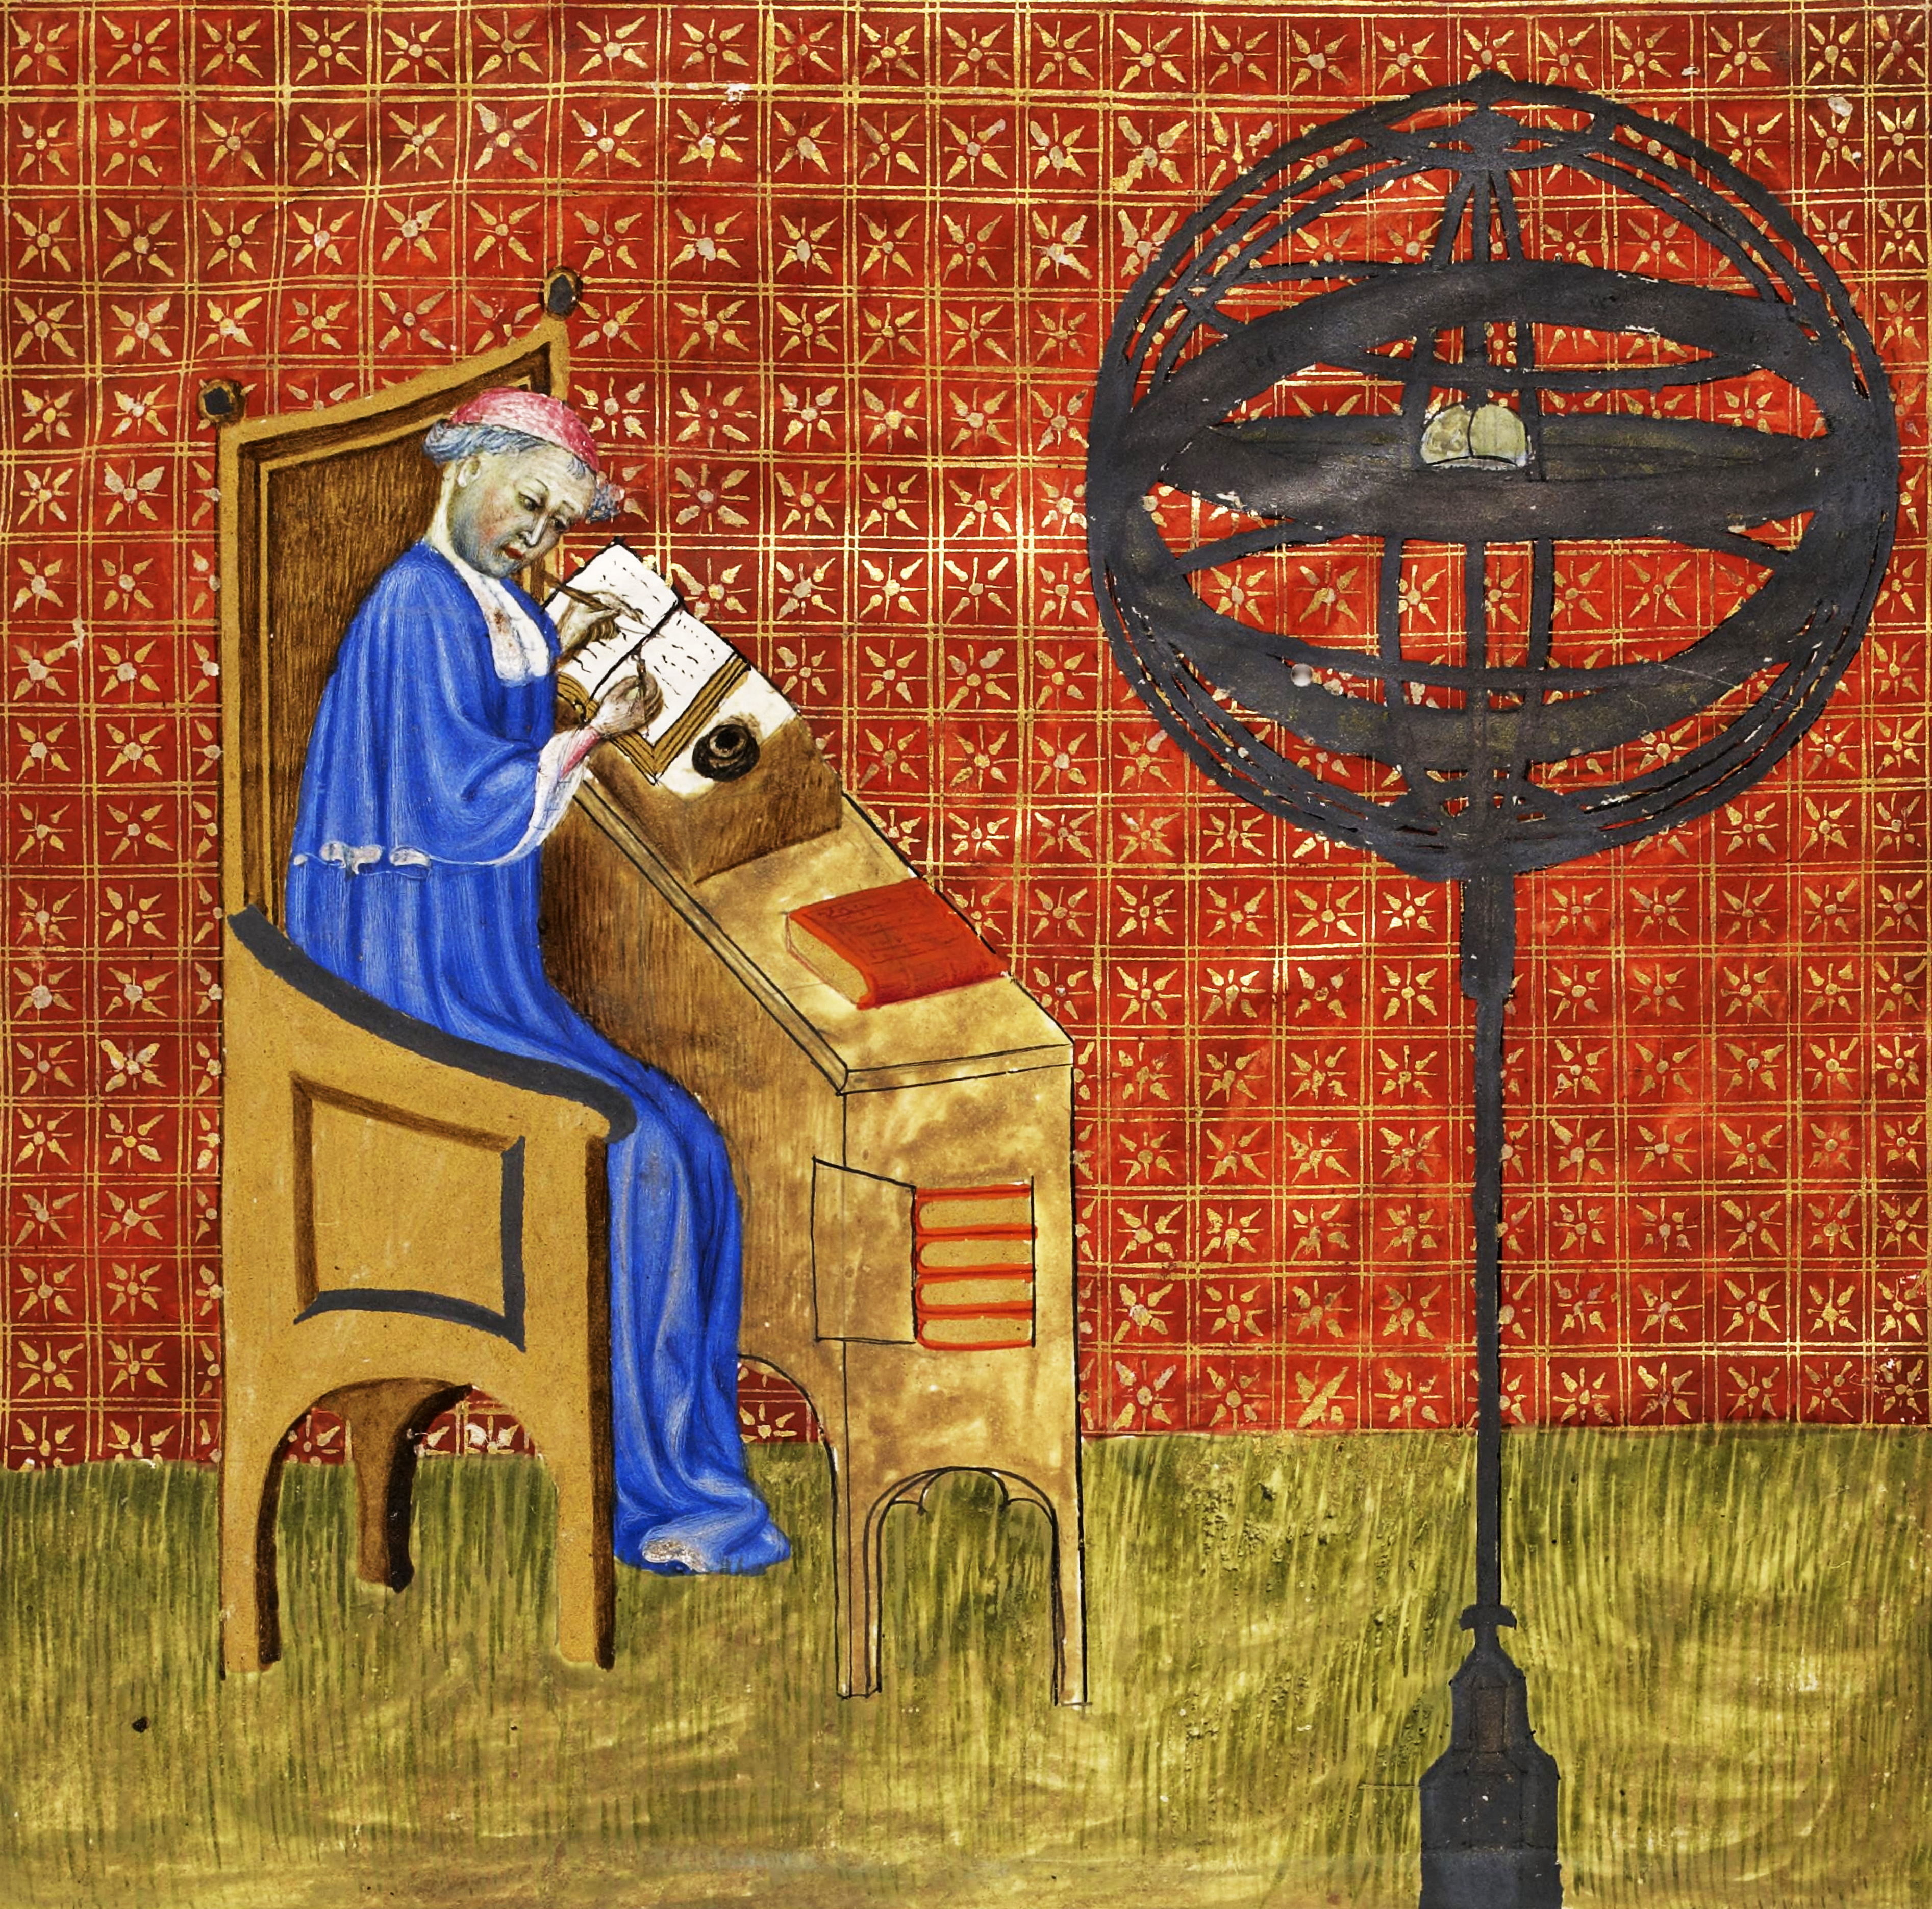
\includegraphics[scale=.25]{a20111203MentalDeath-img001.jpg}
\end{wrapfigure}
Gornahoor places the fateful junction of Western intellectual history at Francis Bacon\footnote{See Section~\ref{sec:BaconModernity} in this book.}. It was Bacon's head-on assault against metaphysical knowledge (``useless knowledge'' that is not power) which signaled Western intention to abandon the medieval project wholesale. Although at various times and places, other movements had been made, Bacon's \emph{New Atlantis} was more completely ``modern''\footnote{\url{http://plato.stanford.edu/entries/francis-bacon/}} and also more suited to corrupt its age. Bacon (for instance) uses ``Magic'' to refer to applied science \& technology, while ``Knowledge'' becomes essentially what we mean today as ``Science''. Blake's ``dark, Satanic mills'' were seen, prophecied, \& invoked by Bacon, and in their present form. Other ``seers'' had conjured up similar forms, but Bacon was seminally specific. Bacon's project (for instance) is innately inherent in William of Ockham's denial of universals. Richard Weaver writes\footnote{\url{http://www.nyx.net/~kbanker/chautauqua/consequences.html}}:

\begin{quotationx}
Surely we are justified in saying of our time: If you seek the monument to our folly, look about you. In our own day we have seen cities obliterated and ancient faiths stricken. We may well ask, in the words of Matthew, whether we are not faced with ``great tribulation, such as was not since the beginning of the world.'' We have for many years moved with a brash confidence that man had achieved a position of independence which rendered the ancient restraints needless. Now, in the first half of the twentieth century, at the height of modern progress, we behold unprecedented outbreaks of hatred and violence; we have seen whole nations desolated by war and turned into penal camps by their conquerors; we find half of mankind looking upon the other half as criminal. Everywhere occur symptoms of mass psychosis. Most portentous of all, there appear diverging bases of value, so that our single planetary globe is mocked by worlds of different understanding. These signs of disintegration arouse fear, and fear leads to desperate unilateral efforts toward survival, which only forward the process.

Like Macbeth, Western man made an evil decision, which has become the efficient and final cause of other evil decisions. Have we forgotten our encounter with the witches on the heath? It occurred in the late fourteenth century, and what the witches said to the protagonist of this drama was that man could realize himself more fully if he would only abandon his belief in the existence of transcendentals. The powers of darkness were working subtly, as always, and they couched this proposition in the seemingly innocent form of an attack upon universals. The defeat of logical realism in the great medieval debate was the crucial event in the history of Western culture; from this flowed those acts which issue now in modern decadence.

One may be accused here of oversimplifying the historical process, but I take the view that the conscious policies of men and governments are not mere rationalizations of what has been brought about by unaccountable forces. They are rather deductions from our most basic ideas of human destiny, and they have a great, though not unobstructed, power to determine out course.

For this reason I turn to William of Occam as the best representative of a change which came over man's conception of reality at this historic juncture. It was William of Occam who propounded the fateful doctrine of nominalism, which denies that universals have a real existence. His triumph tended to leave universal terms mere names serving our convenience. The issue ultimately involved is whether there is a source of truth higher than, and independent of, man; and the answer to the question is decisive for one's view of the nature and destiny of humankind. The practical result of nominalist philosophy is to banish the reality which is perceived by the intellect and to posit as reality that which is perceived by the senses. With this change in the affirmation of what is real,, the whole orientation of culture takes a turn, and we are on the road to modern empiricism.
\end{quotationx}

Conservatives quote Weaver all the time, but nobody takes this seminal passage seriously (or indeed, seems to have read him attentively at all). George Heart in \emph{Dogmatic Faith \& Gnostic Vivifying Knowledge} actually suggests that Aquinas represents a ``first compromise'' by way of Aristotle's influence. Although Hylomorphism is a far cry from modern empiricism, it was a first step:

\begin{quotex}
Although Albertus Magnus himself started to work at amending Aristotle's most conspicuous aberrations, he could never bring his work to completion, and he left the rest of that impossible task to his disciple Thomas Aquinas. We say ``impossible'' because we fully know now that Plato and his unfaithful disciple who betrayed his teachings after having spent 20 years in the Academy could never be reconciled. Origen was right when he said that Aristotle was simply a traitor.

\end{quotex}
Heart thinks that Aquinas betrayed Aristotle to attempt to synthesize Plato \& his wayward student, but others were not so discriminating; Catholics should not forget that in 1210, the Church found it necessary to issue a condemnation of indiscriminate use of Aristotle, Averroes, and Avicenna. The threat from combining things that ought not to be combined was ``sterile heterogeneity'', such as can be found in St. Anselm (1033-1109).

As GK Chesterton noted\footnote{\url{http://distributistreview.com/mag/2011/12/two-difficulties/}}, the big task (exoterically) of our present generation is to conduct committees of correspondence in order to lay the groundwork for understanding what was lost, and why. A scope for action is very limited, but this is to simply put us in the same position as those who created the avenues of decay all those centuries ago – we will be forced to rethink: a man in prison has time for reflection, at last.



\flrightit{Posted on 2011-12-03 by Logres }

\begin{center}* * *\end{center}

\begin{footnotesize}\begin{sffamily}



\texttt{Michael on 2011-12-03 at 14:59 said: }

Outstanding post. What authors do you recommend to start us on the task?


\hfill

\texttt{Logres on 2011-12-04 at 00:41 said: }

Well, one has to remember that the ``Greater Struggle''

\url{http://www.gornahoor.net/?p=3005}

takes precedence, even for the fighter or the peasant, whomever they are. Because of this, Tomberg's book has to be a good place to begin the arts of transformation of the self; Tomberg represents a continuation of the Inkling's insight that the moral universe is opened by the imagination – that is, it is a key, because it lets us out of the modern prison. But it isn't an end in and of itself, contra the poets. I would suggest that a Westerner include a certain familiarity with the enemy – even Orthodox monks in America study Nietzsche, if for nothing else than to help ``see through'' flimsy arguments supposedly made on that very basis. It would be interesting to know (for instance) where Bacon got his ideas (that was discussed a little on that post). Beyond that, I would say ANY book that helps recover the link between Christendom and the Greco-Roman/Nordic heritage is a priceless asset, and in this sense, it hardly matters where one starts. For those who are contemplative, Augustine's Confessions or Boethius' Consolation (my favorite). The dialogues of Plato are read by very few people, and Platonism is a strong antidote to nominalism/empiricism in all its forms. It teaches good mental hygiene. Any historical work that recasts the data into an unfamiliar but plausible shape (eg., Polyani's Great Transformation which debunks the golden mythos of modern capitalism to a great degree) can be useful for purging mental parasites that swarm around us on the TV, in the papers, etc. Anything to set the mind to actually ask itself questions and answer is useful. The turning point for me was realizing how bad the Reformation was, in so many ways:

\url{http://jcrao.freeshell.org/LouisVeuillotReevaluation.html}

Tarapelli is another good Catholic political writer, as is Cortes.

Sir John Polkinghorne has done some thoughtful writing on the implications of quantum physics for religion, and vice versa, although he is not a ``traditionalist'' – he is, however, an independent thinker and someone who actually ``counted'' in the history of physics. It depends upon your field of interest, your temperament, and whether you want to be a scholar, a man of letters, or a fighter. Dante's political treatise on De Monarchia is reliably good, I've been told. And there is a whole slew of new scholarly works, compilations, editions, etc. out there, such as Glenn Magee's new study on Hegel \& Hermeticism, which places an old Leftist favorite in a brand new light. We have to transmute, or undo, what has been done. Perhaps someone should study Bacon and trace how and where he got his concepts and twisted them, in what ways and by what means they shadow and parody truth. They wouldn't be so powerful unless they contained some measure of the truth, even to be powerful in the debased way they are. Remember what Cologero has quoted before – ``the errors of the great are more interesting than the rightness of the small''. Alchemy is important because I think that is what modern science parodies, or apes. Someone could do worse than begin to follow in Franz Bardon's footsteps, and read what he wrote about the Kabbalah, etc. But beyond that, any book which ``calls'' to you in your personal quest for truth, your hunger to escape the prison, is going to help you, by inexorable laws, even if negatively. Following footnotes can sometimes lead you in that quest. If you are specifically interested in Science \& Religion's interaction, I can be more specific. Or if you tell me anything more of where you're coming, I can also be a little more specific. Personally, I need to read Evola on the Grail and his work on magic. I also need to finish Tomberg's Meditations, which are fabulous. What are your favorite books, and what is your ``read before I die'' list?


\hfill

\texttt{Charlotte Cowell on 2011-12-04 at 12:36 said: }

I also love MoTT, it's far and away my most well-used book. I also love Sufi poetry – Bird Parliament, Rumi and the Rubaiyat of Omar Khayyam – and of course The Prophet by Khalil Gibran is a magical masterwork that even a child could read. The Master and Margarita is probably by favourite novel and Carlos Castaneda inspired me to become conscious in dreams. Whether fact or fiction, his journeys with Don Juan certainly fire the imagination. A Midsummer Night's Dream is my favourite Shakespeare play (or Bacon play as some of you probaby think!) and Yeats is one of my favourite poets. Von Balthasar's Prayer is one of the best tools for helping one to learn contemplative prayer that I know of and certain parts of Augustine's confessions have touched me very deeply and 2 Corinthians 6 is my favourite part of the Bible. From the Greeks I love the dramas and Orphic Hymns. More recently The Discovery of Heaven by Harry Mulisch is amazing (as is the film of the same name), but the best thing I ever EVER read in my life was a love poem written by God for the lost Divine feminine which generated the universe so he could try to find her :-)


\hfill

\texttt{logres on 2011-12-04 at 17:08 said: }

Charlotte, what do you mean, conscious in dreams? Waking up inside of them?


\hfill

\texttt{logres on 2011-12-04 at 17:11 said: }

I should also say that Chesterton and Belloc thought (think) that those who can, should go back to the land, in one way or the other. This gives an existential, practical base to the struggle which permits more independence of thought, than (say) someone whose opinions (if known) could affect their employment. Evola is still the best Western introduction for many people, I would think? Gornahoor has a lot of his essays here – the one on Falangism is good, as well as Reincarnation.


\hfill

\texttt{nous on 2011-12-04 at 17:12 said: }

Placing the cosmos in philosophical terms represents the first fall or any dialectics that could elicit an opposite reaction, outside even of historiography. Somewhere at the point of paradisaical origins authority was over-ruled. But let me echo Micheals question: ``Moar sauce.''

Indeed, I commend you Logres on those examples given but what of the action orientated spirit? What recommendations can be given to those who wish to follow a direct path of the fighter (striking both inner and greater battles). I would like you or any member of the Gornahoor staff to address this important question.

I have read Franz Bardons books(achieving the goals therein if even possible beyond the 4th level is another question). Evola's operative methods in ``Introduction to Magic'' and ``Yoga of Power'' are intriguing but not final. Catholicisms mortification of the flesh is another tempting facet, as is that of the Buddhist/Zen response to ``no mind'' and to the perfection of ones actions. What is needed is real life engagement which is what I believe O.D founder St Jose-maria Escriva had in mind to the inter-war period of decadence he found himself in.


\hfill

\texttt{Charlotte Cowell on 2011-12-04 at 19:27 said: }

Yes, Don Juan's teaching to Carlos about dreaming, is in fact a useful method for learning how to `wake up’ – to become conscious with will and mind – in a dream. The Indian tells his pupil he must strive to see his own hands in a dream, which takes the pupil a long time. It took me ten years, although I had out of body experiences often, in both the lower and higher astral, but not of my own volition until this one time. Basically one conditions one's self to associate seeing the hands with being conscious, it's a form of inner programming. Actually one could choose anything, it's the technique that's important in this case rather than the particular, as I understand it. One might equally decide to see one's feet I suppose. When this happened to me (ie, I saw my hands), firstly I note they looked very strange to me, being whiteish grey and translucent in that state it led to the vision of Genesis I mentioned above: 

\url{http://alchemical-weddings.com/alchemical-weddings/tunnel-vision}

\url{http://alchemical-weddings.com/alchemical-weddings/rainbow}

more generally, the shamanic training helps to hone the faculties necessary for fruitful spiritual work, such as concentration, self discipline, dedicated endeavour, right motivation, discernment etc.


\hfill

\texttt{Charlotte Cowell on 2011-12-04 at 19:31 said: }

I agree with Chesterton and Belloc by the way, that's why I'm off to Guatemala in February to build a house, farm the land, keep bees etc….

\url{http://www.greennewworld.org/}

it's the only way forward unless we want Earth to become an inorganic sort of hell with half human half robots, weird animal hybrids, totally polluted environments etc. It'll happen sooner than people think if there isn't a significant mass turnaround in terms of commitment to saving the world


\hfill

\texttt{logres on 2011-12-05 at 19:06 said: }

I think I may defer to Cologero on your question, Nous (and Michael, if there was more). My path is intellectual fighting, when it comes to initiative. It is difficult for me to recommend ``when'' or ``how'' unless it is already clear. You are essentially ( I think) wanting an order, something that will require special gifts to institute. If I was going to recommend something, Coudreanu's Legion of the Archangel Michael might be a good place to start. It would be interesting to examine this movement in a dispassionate sense, and to parallel this study with more research along Evola's lines. I am not qualified to state anything further.


\hfill

\texttt{logres on 2011-12-05 at 23:04 said: }

I hate adding to my essay, but I should devote something to this man:

\url{http://truerestoration.blogspot.com/2008/10/book-review-liberal-illusion-by-louis.html}

I don't think any effective rebuilding can occur until the insights of Christian theology are yoked with metaphysical insight (which necessarily draws on pagan elements). Essentially, as Charlotte has pointed out, this is a matter of connecting dots in every sense of the word, which is Cologero's ambitious and noble project. If Catholic dogma could be transmuted/translated into metaphysics, and vice versa, by an elite, then the path of the fighter is made much easier, and less subject to disastrous mistakes as they struggle to bore back into their heritage from the outside. So long as one individual ``hears the music'' and does not bow the knee to Baal or any lesser gods, the world exists for him/her. That being would be sovereign. Like a soul who battles to save the body, or a spirit, the soul, so would that one person fight to inherit the world called earth for the Pantocrator. They would be the viceroy.


\hfill

\texttt{Charlotte Cowell on 2011-12-06 at 06:09 said: }

Yes, we have to know where we came from to really know where we're going – the past proceeds from the future as much as the future proceeds from the past. When I was first converted to Christianity I discovered a sublime unity – and no conflict – with classical religion, but also Buddhist and Sufi principles in a truly universal sense. Problems might come via the reincarnation doctrine, which might cause one to redevelop a soul attachment to the `old ways'. then trauma when this is necessarily severed. However consciousness of the hows and why helps make this easier to bear and it is not so difficult to put those kinds of memories back into the realm of imagination.


\hfill

\texttt{Gabe Ruth on 2011-12-06 at 10:10 said: }

Thanks for this, it really got my blood racing. For those more action oriented, John Robb (writes Global Guerrillas) is very interesting and somewhat practical. Though I've never seen him comment on metaphysics himself (has linked to others of this bent on occasion), his thoughts on how far wrong we have gone and where we need to go jive with the ideas around here with regards to worldly steps. The whole resilient community is worth a look, though they are generally not cognizant of metaphysics.


\hfill

\texttt{logres on 2011-12-06 at 22:37 said: }

That's a good point about ``time flowing backwards''.


\hfill

\texttt{logres on 2011-12-06 at 22:38 said: }

I've heard of John Robb, \& will look him up, thank you.


\hfill

\texttt{Perennial on 2011-12-08 at 03:51 said: }

I recommend anything on the Action Francaise, which works were so action-packed I became a traditionalist just from reading a history of it! The Camelots du Roi, their seminars, their newspaper and of course the pivotal Charles Maurras were all inspirational. The Legion is excellent also, and of course anything related to the Carlists of Spain is great, although I know of only 2 works in English. These were all action-based movements (Action Francaise says it all) and therefore an excellent study for those who wish to benefit from them as well as to attempt to rectify their shortcomings.


\hfill

\texttt{Charlotte Cowell on 2011-12-08 at 14:58 said: }

`If Catholic dogma could be transmuted/translated into metaphysics'

Does Rudolf Steiner go some way towards achieving this? Granted he is elliptical and strange, but he was pretty ahead of his time all the same….

Apart from that, I think this is a matter that is wholly dependent upon subjective experience, because without that one would not necessarily recognise the analogies in philosophical/theological works. Even then it depends on `right place and right time'. I might read something one day that means nothing, but ten years later speaks volumes (or indeed vice versa). 

In terms of a catholic theologian who regularly speaks volumes, von Balthasar I find outstanding. Recently this aphorism from his `A grain of wheat'. helped me to understand a very particular spiritual `problem' or `question' I had pertaining to one experience in particular that was both very upsetting and something for which i felt unaccountably (but profoundly) grateful. At the time I viewed it as being a certain spiritual death, so the gratitude was difficult for me to comprehend, although I did at the same time `see' something akin to fireworks going off deep in outer space so assumed it was an occasion for some form of celebration. The extract is on my blog (it is short):

\url{http://alchemical-weddings.com/alchemical-weddings/integration}


\hfill

\texttt{logres on 2011-12-08 at 23:52 said: }

Charlotte, here is a quote from what you posted:

``But if no understanding is developed, if this particular faculty is stamped out, if those who speak about faculties of this kind are put away as if they were insane, disaster in inevitable and humanity will sink in the morass of materialism. Everything will depend upon whether understanding is awakened for Spiritual Science, or whether Ahriman will succeed in suppressing its intentions…''

I've linked to Bondarev's interpretation of Steiner, which removes some of the necessary detritus and evolutionary Zeitgeist which adheres to Steiner's work (which Cologero has quite properly drawn attention to). This is almost a quote of St. Anthony – ``in that time, when men go mad, they will find him who is not mad, and call him mad''. Isn't this where we have arrived at? Even Phillip Rieff (a total ``secularist'' \& Jew) could see this quite clearly. Goethe also prophecied it – ``we will all take care of each other in hospitals''. The stench of the mental sick bed is all around us. But I think Steiner is a piece of the puzzle, provided someone can interpret him in a less ``spiritualist'' viewpoint, although the ``spiritualist'' viewpoint had more traditional elements, then. So I think this is right, your insight here.


\hfill

\texttt{Charlotte Cowell on 2011-12-09 at 05:37 said: }

In answer to this question:

``in that time, when men go mad, they will find him who is not mad, and call him mad''. Isn't this where we have arrived at?''

No, I think we have just been there and that now the network of the `non mad’ – ie, the pioneers – have collectively `fought off' the assault, so to speak, and have consolidated their forces. Just. It's very early days but we're on the way back up now because a critcal mass of `seers and believers' has been reached. Only just! it's inconceivable that once the universal tipping point has been reached we'll collectively fall back into the abyss – we went through the abyss to ensure we won't go there again en masse. 

Metaphorically speaking, enormous numbers of people are loaded onto the `Mother Ship' ready for take off, mostly without realising it!

I do think, however, that perhaps more than ever these are days for prayer and focus on the joyful and luminous mysteries.


\hfill

\texttt{Charlotte Cowell on 2011-12-09 at 05:41 said: }

By the way I am not a diehard fan of Steiner – I agree with many of the well known reservations – it's just that I can see that he could see and am only recently starting to understand how he presented his information. He relentlessly spoke to the developing spiritualised being in us all and was fearless in risking being wrong in order to be right! Crazy wisdom….


\hfill

\texttt{Boreas on 2011-12-09 at 08:35 said: }

Charlotte, I think you are right about the fact that ``a critical mass of seers and believers'' has been reached and we're heading towards a new upward pointing cycle in the longer run, but despite – and because of! – this, the current world-age is in its death throes and the world is on the verge of a third planetary cataclysm in the short run. No utterance for world peace etc. can change this fact, no matter how good-willed a man or a woman might be. (I think you know this also and this was not exactly what you were referring to, but as an semi-official voice of cosmic pessimism I had to say this!)

Here's the true ``beef'' of the matter: this is not a call for panic, anguish and despair, but for hope and joy. Things couldn't be otherwise than they are. The divine spirit of man is awakening again from its slumber and THIS is the very thing that is the primal cause of all that's happening – even in its negative manifestations.


\hfill

\texttt{Charlotte Cowell on 2011-12-09 at 09:12 said: }

Boreas yes, I think we are in agreement and I am in the mode now of being positive. I stared into the abyss from 2009 – 10 and at the time I wondered how people would cope with what was to come, if it proved so devastating to me personally, for all my faith and hope in `other things'. Clearly we are in a time of major, enormous change – an `anything goes' type of situation in which all the birds are coming home to roost. The relief comes from the fact that karma is finally being faced, because as you point out, we can't move on with the new until we've moved on from the old. However I don't see that there is a need to throw the baby out with the bathwater, and we should always bear in mind that the heavenly quality of mercy `wins' in the end. This is why prayer is still so important. I firmly believe that we should all be praying for mercy and redemption – for both self and others – on a daily basis now, as to do less would be to deny the possibility of damage limitation. Anything is possible.

There is something on my blog here about Prayer/Benediction:

\url{http://alchemical-weddings.com/alchemical-weddings/act-of-benediction}


\hfill

\texttt{Charlotte Cowell on 2011-12-09 at 09:31 said: }

\url{http://beforeitsnews.com/story/1483/117/Pope\_Highlights\_Marys\_Role\_As\_Woman\_Of\_The\_Apocalypse.html}


\hfill

\texttt{Boreas on 2011-12-10 at 10:45 said: }

You are of course right Charlotte. I never meant to mean that prayer is futile or hoping for a peaceful solution to world problems is in vain / naïve. On the contrary, I think these are the very duties of spiritual or religious people in these times.


\hfill

\texttt{Golgonooza on 2011-12-12 at 12:04 said: }

Thanks for the post, especially the link to the Richard Weaver writing, which was fascinating. Thanks also Charlotte, for the Von Balthasar aphorism; as usual you have brought something to my awareness which chimes with what I'm currently pondering!


\end{sffamily}\end{footnotesize}
